\documentclass[a4paper,10pt]{article}

\usepackage[margin=2cm]{geometry}
\usepackage{graphicx}
\usepackage{amsmath}
\usepackage{array}
\usepackage{hyperref}
\usepackage[all]{hypcap}
\usepackage{listings}
\lstdefinestyle{TerminalStyle}{
  language=bash,
  basicstyle=\small\sffamily,
  numbers=left,
  numberstyle=\tiny,
  numbersep=3pt,
  frame=tb,
  columns=fullflexible,
  linewidth=0.9\linewidth,
  xleftmargin=0.1\linewidth
}
\lstdefinestyle{HtmlStyle}{
  language=html,
  basicstyle=\small\sffamily,
  numbers=left,
  numberstyle=\tiny,
  numbersep=3pt,
  frame=tb,
  columns=fullflexible,
  linewidth=0.9\linewidth,
  xleftmargin=0.1\linewidth
}
\lstdefinestyle{OutputStyle}{
  language=html,
  basicstyle=\small\sffamily,
  frame=tb,
  columns=fullflexible,
  linewidth=0.9\linewidth,
  xleftmargin=0.1\linewidth
}

\setlength{\parindent}{0pt}
\setlength{\parskip}{1ex plus 0.5ex minus 0.2ex}

\title{
\includegraphics[width=12cm]{Eeufeeslogo.jpg} \\
       Department of Computer Science \\
       University of Pretoria \\
       \vspace{0.5cm}
       Software Engineering\\
       COS301 \\
       \vspace{0.5cm}
       \begin{large}Peer Introduction to Software Engineering Concepts\end{large}
}

\date{} 
\author{Broekman, A (Andrew) \\
U11089777}

\begin{document}
\maketitle

Congratultions, if you are reading this, it means that you have successfully cloned the Team Echo git repository. This document introduces you to some software concepts necessary for completion of the COS 301 mini project. In the process you will gain valuable skills to be used in industry and academia, setting you apart from fellow colleagues. This document provides you with practical tasks to complete, and you are urged to complete these tasks, as we know, the only way to learn in programming is to DIY (Do It Yourself). 

\section{Git}
\subsection{Git}

Git is a distributed version control system or so called source code management system developed by Linus Torvalds in 2006 for managing the Linux kernel source code. Git is distributed, meaning that each developer has the complete repository history, independent of network access. This means, that even when you are offline, you still work on your code. It is important to note that Git and Github and also Git and Bitbucket are not the same. Git is the client used on your machine to manage your repository and keep a record of what changed in your code. Github and Bitbucket are services provided to the internet, to allow people to upload there Git repository onto a public server. Thus, you can view Git similar to Photoshop, you create your own graphic files and keep them on your local PC. However when you want to share your files with friends, you may want to upload your files to a cloud service such as Dropbox, Google Drive, Microsoft OneDrive etc.

\subsection{Installing git on Ubuntu}

To install the git client on Ubuntu, one would use the following commands in a terminal \\
\begin{lstlisting}[style=TerminalStyle]
# sudo apt-get update
# sudo apt-get install git
# git config --global user.name "Your Name"
# git config --global user.email "youremail@domain.com"
\end{lstlisting}

\subsection{Installing git on Windows}

For installation of git on Microsoft Windows, the easiest is to use one of the following software packages

\begin{enumerate}
\item Github for Windows\\
This is a CLI and GUI git software package released by Github.com.  More information is available at \url{https://desktop.github.com/}
\item Offical Git Client for Windows\\
This is the offical Git client for Windows. More information is available at \url{https://git-scm.com/downloads}
\end{enumerate}

Replace \textbf{Your Name} and \textbf{youremail@domain.com} with your own name and email address you used to register on Github, making sure to surround both in quotations.

\subsection{Introduction to Git}

For this part of the tutorial we will be using the git terminal, as this will allow you to understand the concepts much better.

Create a new directory called \textbf{cos301tutorial} in your home directory.
\begin{lstlisting}[style=TerminalStyle]
# cd ~
# mkdir cos301tutorial
# cd cos301tutorial
\end{lstlisting}

We will now create a new empty git repository in the \textbf{cos301tutorial} directory.
\begin{lstlisting}[style=TerminalStyle]
# git init
\end{lstlisting}

Now the real fun begins. Create a new file, called \textbf{index.html}, adding only the html opening and closing tags.
Your index.html file should now look like this
\begin{lstlisting}[style=HtmlStyle]
<html>

</html>
\end{lstlisting}

In the terminal, issue the following command, 
\begin{lstlisting}[style=TerminalStyle]
# git status
\end{lstlisting}

You should receive output similar to the following:
\begin{lstlisting}[style=OutputStyle]
On branch master

Initial commit

Untracked files:
  (use "git add <file>..." to include in what will be committed)

	index.html

nothing added to commit but untracked files present (use "git add" to track)
\end{lstlisting}

Notice that git indicates that the index.html file is not tracked. This means that any changes you make, will not be recorded in the git history. Therefore when you create a new file, which should be tracked in git, it is important to ensure you add this file to git. 

Do note, that we never commit and file that can be regenerated from other commited objects in the repository. Examples of such files are compiled class files, object files, executables, compiled pdf documents, auxiliary and log documents from \TeX{} or \LaTeX{} compilation. This is the reason for the .gitignore file, which you are encourage to view and read more about, as any developer worth there salt will make use of a .gitignore file. A nice Git repository exists with gitignore files for multiple tools, languages, OS's etc., which assists developers in ensuring only the needed files make it into the repository. For more information refer to \url{https://github.com/github/gitignore}

To add this new file to git we use the command, 
\begin{lstlisting}[style=TerminalStyle]
# git add index.html. 
\end{lstlisting}

This now brings us to the three sections of a git project, the working directory, staging area, and Git directory as show in figure~\ref{fig:gitareas}.

The Git directory, normally stored as a hidden directory, .git, in your root directory of your project, is the database of your repository. Git stores all files, also know in the git world as objects, as well as metadata in this directory, and it is this directory that is copied when you cloned the Team Echo repository from Github.

The working directory, is a single checkout at one point in time. When you checkout a specific version of your project, the files are decompressed from the .git directory and extracted into the root project directory, allowing the developer to use and modify the files.

The staging area is an intermediate holding area, internally represented as a file, which contains information about what changes will go into your next commit. The staging area allows one to queue more than one change to go into a commit, which allows developers to cluster groups of changes together. Some literature refers to the staging area as the index.

The git workflow works as follow:

\begin{enumerate}
\item You create, modify and delete files in your working directory
\item The changed files, which included files which have been created and deleted, are then added to the staging area. This means snapshots are added to the staging area.
\item The staging area is then commited, which takes the snapshots of the files as they are in the staging area, and adds it into the git database.
\item Wash and repeat
\end{enumerate}

\begin{figure}[h]
\centering
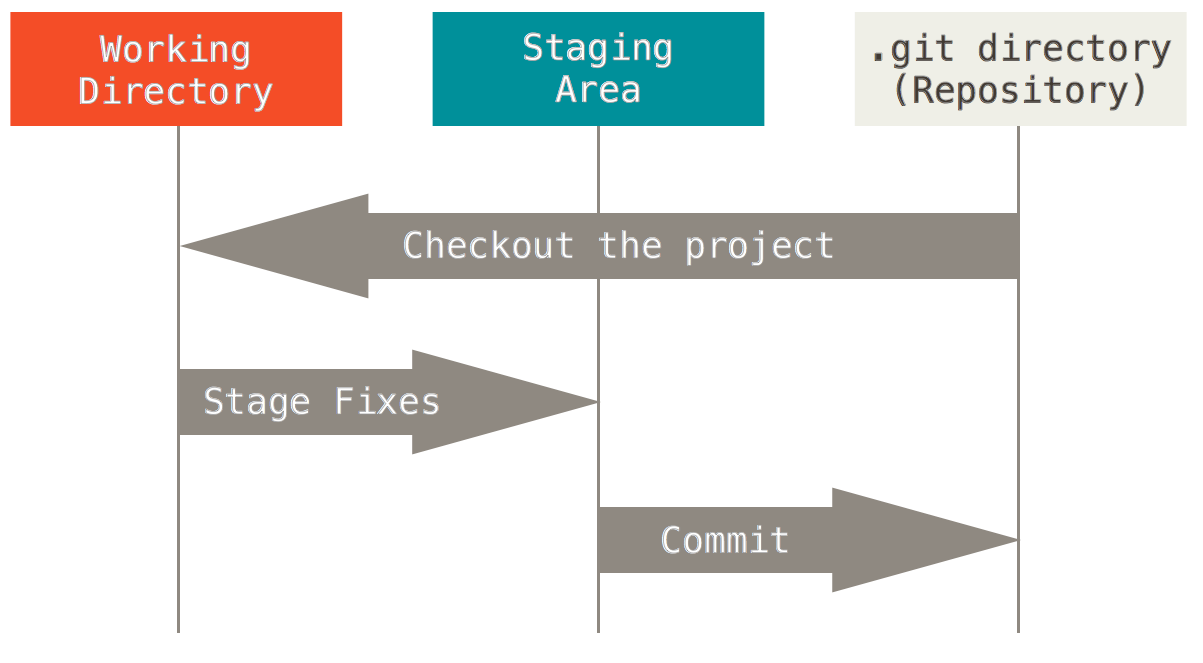
\includegraphics[scale=0.3]{areas}
\caption{Working directory, staging area, and Git directory.
 (Source: \url{https://github.com/progit/progit2/blob/master/book/01-introduction/images/areas.png})}\label{fig:gitareas}
\end{figure}


Your index.html file is now in the staging area. Lets finish off by adding this file into the git database, by using the command 
\begin{lstlisting}[style=TerminalStyle]
# git commit -m "Creates a new empty HTML file". 
\end{lstlisting}

Note that git allows one to attach a message to a commit, which allows other developers and yourself in the future to understand what changes a certain commit has made to your source code. As part of self documenting code, communication and understanding by other developers what you did, it is very important to write clear and concise messages of what changes a commit introduces to the source code.

The power of git will now be unleashed. Branches in git allows one to work seperatly from production ready code, allowing one to experiment, add new features, correct bugs etc. Create a new branch called headBranch
\begin{lstlisting}[style=TerminalStyle]
# git branch headBranch
\end{lstlisting}

Git has now created a new branch, called headBranch, lets go ahead, and switch to this branch now by using the command,
\begin{lstlisting}[style=TerminalStyle]
# git checkout headBranch
\end{lstlisting}

We can ensure that we are on the correct branch by using the command 
\begin{lstlisting}[style=TerminalStyle]
# git status
\end{lstlisting}

From the output below you will notice that git indicates \textbf{On branch headBranch}.
\begin{lstlisting}[style=OutputStyle]
On branch headBranch
nothing to commit, working directory clean
\end{lstlisting}

Go ahead, open the index.html file, and add a html head tag, i.e. you file will now look like this
\begin{lstlisting}[style=HtmlStyle]
<html>
<head>

</head>
</html>
\end{lstlisting}

We will now add this file to the staging area, and commit it. Issue the following commands
\begin{lstlisting}[style=TerminalStyle]
# git add index.html
# git commit -m "Adds head tag to file"
\end{lstlisting}

We will now checkout the master branch, by using the command
\begin{lstlisting}[style=TerminalStyle]
# git checkout master
\end{lstlisting}

Go ahead and open your index.html file. Shock ... ... ..., there is no head tag. I know, quite shocking, but it is correct. This is one of the most powerful features of git, when you want to experiment on your own code, test some stuff, without breaking it, you can always create a new branch to test your crazy experiments, and throw the branch away if it doesn't work. However, should your code work, you can always add your new changes to your old code, but we are jumping ahead.

We will now checkout a new branch, called bodyBranch and add the body tags to the index.html file. You can repeat the same procedure as was done for the headBranch, just replaceing the word head with body. However, if you are unsure here are the commands
\begin{lstlisting}[style=TerminalStyle]
# git branch headBranch
# git checkout headBranch
\end{lstlisting}

 Before you commit your code, make sure that your index.html file looks like this:
\begin{lstlisting}[style=HtmlStyle]
<html>
<body>

</body>
</html> 
\end{lstlisting}

\begin{lstlisting}[style=TerminalStyle]
# git add index.html
# git commit -m "Adds body tag to file"
\end{lstlisting}

After you have commited your code, we will switch back to the master branch again, using 
\begin{lstlisting}[style=TerminalStyle]
# git checkout master
\end{lstlisting}

We will now update our file on the master branch, add a DOCTYPE declaration to the file. Ensure your index.html file looks like this, before commiting.
\begin{lstlisting}[style=HtmlStyle]
<!DOCTYPE html>
<html>

</html> 
\end{lstlisting}

Add this file to the staging area and commit it with a message of "Added DOCTYPE declaration".
\begin{lstlisting}[style=TerminalStyle]
# git add index.html
# git commit -m "Added DOCTYPE declaration"
\end{lstlisting}

We will now use the power of git to combine all your hardwork to create a complete html document. Important to note, that when one merges git branches, you always merge the branch you give as a terminal paramter into the current active branch, given by git status command. Hence we want to import our work from headBranch into the master branch, hence we need to ensure that we are on the master branch. This can be checked as before by typing 
\begin{lstlisting}[style=TerminalStyle]
# git status
\end{lstlisting}

or using the command

\begin{lstlisting}[style=TerminalStyle]
# git branch
\end{lstlisting}

and ensuring that the master branch has an asterisk on the left hand side of it's name. This indicates that it is the current active branch.

To merge the headBranch into the master branch issue the command
\begin{lstlisting}[style=TerminalStyle]
# git merge headBranch
\end{lstlisting}


Go ahead and open the index.html file. You should notice that you have the following
\begin{lstlisting}[style=HtmlStyle]
<!DOCTYPE html>
<html>
<head>

</head>
</html> 
\end{lstlisting}

As you can see, git was smart enough to have understood how it should combine your files. We will now merge the bodyBranch into the master branch, by using the command
\begin{lstlisting}[style=TerminalStyle]
# git merge bodyBranch
\end{lstlisting}

You will notice that git indicates that it has encounted a conflict
\begin{lstlisting}[style=OutputStyle]
Auto-merging index.html
CONFLICT (content): Merge conflict in index.html
Automatic merge failed; fix conflicts and then commit the result.
\end{lstlisting}

This means that git is not sure how it should combine the file, and hence is not going to proceed, but rather wait for you to tell it how to proceed. If you open your index.html file, you will notice git combinded the files, but is showing you which part of the file came from which branch. 
\begin{lstlisting}[style=HtmlStyle]
<!DOCTYPE html>
<html>
<<<<<<< HEAD
<head>

</head>
=======
<body>

</body>
>>>>>>> bodyBranch
</html>
\end{lstlisting}

It is now up to you as the programmer to indicate to git which parts are correct and how you want the file combined, by editing the file by hand to correct it. In this example, we want all the code, so we simply remove meta data lines such that your file looks like the one given below:
\begin{lstlisting}[style=HtmlStyle]
<!DOCTYPE html>
<html>
<head>

</head>
<body>

</body>
</html>
\end{lstlisting}

We will now add this file to the staging area and commit it, using a message such as "Merges bodyBranch into master branch document".
\begin{lstlisting}[style=TerminalStyle]
# git add index.html
# git commit -m "Merges bodyBranch into master branch document"
\end{lstlisting}

Now, how will the lecturers see that you are a hard worker or social loffer? Easy type 

\begin{lstlisting}[style=TerminalStyle]
# git log
\end{lstlisting}

To see the changes you made, you can use the following command
\begin{lstlisting}[style=TerminalStyle]
# git log -p
\end{lstlisting}

There is all the history of what we have been doing so far, as well as who committed code and at what time the code was checked in.

\subsection{Social side of code sharing}
Head on over to Github.com and create a new repository, called cos301tutorial. AFter creation you will find a similar line to this,

\begin{lstlisting}[style=OutputStyle]
git remote add origin git@github.com:andrewbroekman/cos301tutorial.git
\end{lstlisting}

Copy and paste this line into a terminal. This line will link your repository to the online repository on GitHub. However, we need to upload our git repository to Github, similar to how we upload HTML,CSS and JS files to a webserver using FTP. To upload the files to GitHub, we issue the following command
\begin{lstlisting}[style=TerminalStyle]
# git push -u origin master
\end{lstlisting}

This pushes your master branch code, to the origin server. The origin server is GitHub, as can be seen in the code line below.

\begin{lstlisting}[style=OutputStyle]
git remote add origin git@github.com:andrewbroekman/cos301tutorial.git
\end{lstlisting}

The word origin is just a label which is used as an index to specify the URL of the remote server. Advanced git usuage allows push code to multiple servers. 

You can now go ahead, and explore your repo on GitHub, ensuring you get familiar with the GitHub interface.

Go ahead, and checkout the headBranch again. We will now push this branch also to Github so that your friend can assist you in writing the head section with you. 
\begin{lstlisting}[style=TerminalStyle]
# git push -u origin headBranch
\end{lstlisting}

Go explore your headBranch history on Github.

We can now go ahead and a title tag to the head tag. Also, we create a new file, called README, where you can write all about your new site that you will launch. Ensure your index.html looks similar to this

\begin{lstlisting}[style=HtmlStyle]
<!DOCTYPE html>
<html>
<head>
	<title>COS301 Git Intro</title>
</head>
<body>

</body>
</html>
\end{lstlisting}

My README file looks like this

\begin{lstlisting}[style=TerminalStyle]
That's one small step for [a] man, one giant leap for mankind - Neil Armstrong
\end{lstlisting}

We will now commit multiple files in one go, issuing the following commands

\begin{lstlisting}[style=TerminalStyle]
# git add index.html
# git add README
# git commit -m "Adds title tag and README file"
\end{lstlisting}

Important to note, committing only adds a file to the local repository history, not to Github. You can verify this, by checking the commits in the headBranch to verify that this latest commit was not added to Github. Why, we haven't upload our changes yet, so go ahead and upload your changes.

\begin{lstlisting}[style=TerminalStyle]
# git push -u origin headBranch
\end{lstlisting}

Your changes will now be visible in Github, verify this.

Finally, checkout your master branch or bodyBranch, and see if they contain a README.md file?

\subsection{Why do I need to use branches?}

As noted in class, your master branch should always contain production ready code, i.e. this branch should be able to be checked out anytime of the day or night and be able to compile without errors, and the system should be in a fully working state. To achieve this, we use git branches, to accomplish this, however branches introduce a lot of administration, which we have not done properly in the above tutorial, that should be done before a branch is merged.  Hence based on the following blog post by Vincent Driessen titled "A successful Git branching model" located at \url{http://nvie.com/posts/a-successful-git-branching-model/} spurred the open source community to create a branch management tool for git called called git flow.

To install git flow on Ubuntu
\begin{lstlisting}[style=TerminalStyle]
# sudo apt-get install gitflow
\end{lstlisting}

In your cos301tutorial, issue the following command
\begin{lstlisting}[style=TerminalStyle]
# git flow init
\end{lstlisting}

The above command initiates the git flow tool for this repository. You can go ahead and accept the defaault settings. Refer to this handy cheatsheet \url{http://danielkummer.github.io/git-flow-cheatsheet/}
The nice thing about gitflow, is that it merges the branches in the correct order for you, as well as clean old branches etc. Most git clients today support git flow, as it is widely used in industry.

For a very good tutorial on git flow is presented by GitHub. More information is available at \url{https://guides.github.com/introduction/flow/}

\subsection{COS301 Mini Project Assignment}
Once you are comfortable with git, go ahead and add your details to the CONTRIBUTORS.md file, commit and push your changes to the echo repository.

For more information about git and tutorials, refer to the following links:

\begin{itemize}
\item \url{https://git-scm.com/}
\item \url{http://book.git-scm.com/}
\item \url{https://www.atlassian.com/git/tutorials/}
\item \url{http://gitimmersion.com/}
\end{itemize}


\section{\LaTeX{}}
\subsection{What is \LaTeX{}?}

\LaTeX{} is a document preparation software and document markup language. \LaTeX{} is based on Donald Knuth's \TeX{} typesetting software, and LaTeX itself is written in the \TeX{} macro language. \LaTeX{} differs from traditional word processors, which are based on the WYSIWIG (What You See Is What You Get) principle, rather letting the author focus on the content of the article in question, and leaving styling up to the TeX system. The author can however provide hints and markup certain content to provide the system with more information about the required layout and appearance. 

\subsection{Installing \LaTeX{} on Ubuntu}
To install \LaTeX{} on Ubuntu, issue the following commands

\begin{lstlisting}[style=TerminalStyle]
sudo apt-get update
sudo apt-get install texlive-full
\end{lstlisting}


\subsection{Installing \LaTeX on Windows}
Microsoft Window users can install \LaTeX{} by using the MiKTeX package. More information is available at \url{http://miktex.org/}.

\subsection{\LaTeX{} document}
To see how a \LaTeX{} document looks like, navigate to the Team Echo repository, open the docs folder, whereafter open the intro folder. Next open the tutorial.tex file in your favorite text editor to see how the document looks.

To compile this document, issue the following command
\begin{lstlisting}[style=TerminalStyle]
# pdflatex tutorial.tex
\end{lstlisting}

This will produce a PDF file called, tutorial.pdf.

For more information about \LaTeX{}, refer to the following links:

\begin{itemize}
\item \url{https://en.wikibooks.org/wiki/LaTeX/Introduction}
\item \url{https://latex-project.org/intro.html}
\item \url{http://www.andy-roberts.net/writing/latex}
\item \url{https://tobi.oetiker.ch/lshort/lshort.pdf}
\end{itemize}

Also refer to the support materials section, specifically section~\ref{sec:safaritechbooks}.

\section{Support Materials}
\subsection {JetBrains IntelliJ IDEA Ultimate}
The IntelliJ IDEA IDE from JetBrains is of the most advanced and inteliigent Java IDE's avaiable.  However with the time and resources invested by JetBrains, it is also one of the most expensive IDE's on the market, especially to students, at a cost of US\$ 499.00.  However as students of the University of Pretoria, we are however granted the privilege of obtaining this software for free. 

The reason I recommend this software, is that it has very good support for DI (Dependency Injection) framworks and unit testing frameworks.

To acquire this software, head on over to \url{https://www.jetbrains.com/shop/eform/students}, complete the form and enjoy your new software. To ensure you will be able to get access to the software, ensure in the \textbf{Apply with} section you select \textbf{Univesity email address}. In the email field, use your UP GMail account to register, i.e. \textbf{uXXXXXXXX@tuks.co.za}, where uXXXXXXXX is your student number.

\subsection{Safari Tech Books}
\label{sec:safaritechbooks}
A lot of UP students are not aware that they have free and legal access to over 40 514 technology books. In order to access Safari Tech Books

\begin{enumerate}
\item Naviagte to \url{http://www.ais.up.ac.za/}
\item Move your cursor over the \textbf{E-Resources} tab, allowing the drop down menu to open.
\item Select \textbf{E-Book Collections} - Direct Link \url{http://www.library.up.ac.za/ebooks/collmain.htm}
\item Select \textbf{Safari Tech Books Online}
\item Enter your student number, without the "u" and library password
\item Enjoy your access to free, legal tech books.
\end{enumerate}

For more information on \LaTeX{}, do a search on \LaTeX{}. You will notice this site contains books on all technology topics, from server administrations such as how to setup BIND (DNS server), Java Game development, LaTeX, PHP, Android dev, Java EE, Spring, Scale etc.
\end{document}
